\chapter{Struttura di un compilatore, semantica statica, semantica dinamica}
\section{Vincoli contestuali}
\dfn{vincoli sintattici contestuali}{
    I \text{vincoli sintattici contestuali} sono termini o parole riservate non esprimibili per mezzo di grammatiche libere (perché non possono descrivere vincoli vincoli che dipendono dal contesto) che bisogna evitare di considerare quando si esegue il codice
}

Tradizionalmente i vincoli sintattici contestuali appartengono alla sintassi, ma nel gergo dei $LP$, si intende:
\begin{itemize}
    \item \textbf{Sintassi}: quello che si \red{scrive per mezzo di Grammatiche Libere}
    \item \textbf{semantica} tutto il resto $\dots$
\end{itemize}  

Pertanto \red{i vincoli contestuali sono dunque vincoli semantici, detti di } \textbf{semantica statica} cioè vincoli che possono essere verificati ispezionando il codice \red{senza mandare il programma in esecuzioni}

Il compilatore delega questi controlli di semantica statica alla cosiddetta \textbf{analisi semantica}
\section{Semantica statica}
\dfn{Semantica statica}{
    Per \textbf{semantica statica} si intende l'insieme di quei controlli che possono essere fatti sul testo del programma senza eseguirlo
}
\esempio{
    \texttt{int A;}\\
    \texttt{bool B}\\
    \texttt{A := B} (errore di tipo)
}
\section{semantica dinamica}
Per \textbf{semantica dinamica} si intende una rappresentazione formale dell'esecuzione del programma, la quale può mostrare errori durante l'esecuzione
\esempio{
    \texttt{read(A);}\\
    \texttt{B := $\frac{10}{A}$} (Se $A=0$ si da un errore in esecuzione. F)
}

Staticamente non si può sapere l'errore perché la sua occorrenza \red{dipende dall'input dell'utente che fornirà durante l'esecuzione del programma}

Per implementare una semantica dinamica occorre fornire un modello matematico che descriva indipendentemente dall'architettura su cui il programma viene eseguito, il "comportamento del programma"

\esempio{
    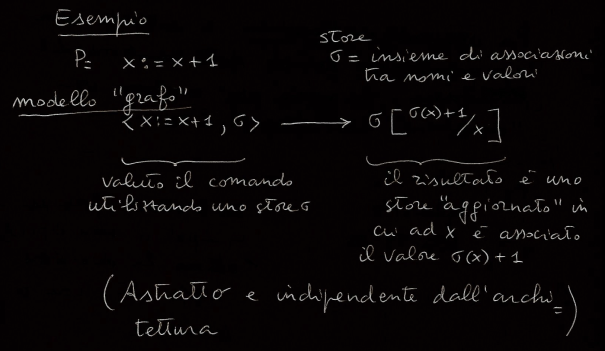
\includegraphics[width=10cm]{esempio_semantica_dinamica.png}
}

\subsection{Utilità della semantica dinamica}
A chi serve la semantica dinamica?

\begin{itemize}
    \item \textbf{Al programmatore}: \textit{ANALISI DEL PROGRAMMA}
    \begin{itemize}
        \item deve sapere esattamente cosa debba fare il suo programma
        \item deve poter dimostrare proprietà del suo programma (ad es.: "termina sempre per ogni possibile input?")
    \end{itemize}
    
    \item \textbf{Al progettista del linguaggio}:
    \begin{itemize}
        \item strumento di specifica del linguaggio
        \item deve poter dimostrare proprietà del linguaggio (ad es.: "è Turing-completo?")
    \end{itemize}
    
    \item \textbf{All'implementatore del linguaggio}:
    \begin{itemize}
        \item riferimento per dimostrare la correttezza dell'implementazione
        
        Infatti \red{un compilatore è corretto quando preserva la semantica dinamica}, quindi per dimostrare che un compilatore è corretto serve avere una semantica per il linguaggio sorgente e per il linguaggio oggetto
    \end{itemize}
\end{itemize}

\subsection{definire la semantica}
Per definire la semantica si utilizzano due tecniche principali: 
\begin{itemize}
    \item \textbf{operazionale}: (macchina astratta a stati e transizioni)
   
    Ovvero si costruisce una specie di automa che, passo a passo, mostra l'effetto dell'esecuzione delle varie istruzioni. \red{vi è una maggiore enfasi su COME si calcola}

    \item \textbf{Denotazionale}: si associa ad ogni programma sequenziale una funzione da input ad output (incluse strutture ausiliarie e memoria). \red{vi è una maggiore enfasi su COSA si calcola}
        
\end{itemize}
\section{Pragmatica nella descrizione di un linguaggio}
\dfn{Pragmatica nella descrizione di un linguaggio}{
    si definisce \textbf{pragmatica nella descrizione di un linguaggio} insieme di regole sul modo in cui è meglio usare le istruzioni a disposizione
}
Esempietti:
\esempio{
    \begin{itemize}
        \item evitare le istruzioni di salto quando possibile
        \item usare le variabili di controllo del \texttt{for}  solo a quello scopo
        \item scelta della modalità più appropriata di passaggio di paramatri ad una funzione
        \item scelta tra iterazione determinata (\texttt{for}) e indeterminata (\texttt{while})
    \end{itemize}
}
\section{
    implementazione
}
\dfn{implementazione}{
    Per \textbf{implementazione} si intende la scrittura di un compilatore per una macchina ospite già realizzata, costruendo così una macchina astratta per il linguaggio
}

\subsection{Correttezza dell'implementazione}

Per far sì che un compilatore sia corretto occorre \red{dimostrare che il programma preservi la semantica}, ovvero il programma sorgente e quello oggetto calcolino la stessa funzione 

\subsection{Struttura di un compilatore}
\begin{tikzpicture}[node distance=1.8cm]

    % Blocchi principali
    \node (start) [process] {Programma sorgente};
    \node (lex) [process, below of=start] {Analisi Lessicale};
    \node (tokens) [process, below of=lex] {Lista di Token};
    \node (syn) [process, below of=tokens] {Analisi Sintattica};
    \node (tree) [process, below of=syn] {Albero di derivazione};
    \node (sem) [process, below of=tree] {Analisi Semantica};
    \node (augTree) [process, below of=sem] {Albero derivazione aumentato};
    \node (interForm) [process, below of=augTree] {Generazione forma intermedia};
    \node (form) [process, below of=interForm] {Forma intermedia};
    \node (opt) [process, below of=form] {Ottimizzazione};
    \node (optForm) [process, below of=opt] {Forma intermedia ottimizzata};
    \node (codeGen) [process, below of=optForm] {Generazione del codice};
    \node (objectCode) [process, below of=codeGen] {Codice oggetto};
    
    % Frecce principali
    \draw [arrow] (start) -- (lex);
    \draw [arrow] (lex) -- (tokens);
    \draw [arrow] (tokens) -- (syn);
    \draw [arrow] (syn) -- (tree);
    \draw [arrow] (tree) -- (sem);
    \draw [arrow] (sem) -- (augTree);
    \draw [arrow] (augTree) -- (interForm);
    \draw [arrow] (interForm) -- (form);
    \draw [arrow] (form) -- (opt);
    \draw [arrow] (opt) -- (optForm);
    \draw [arrow] (optForm) -- (codeGen);
    \draw [arrow] (codeGen) -- (objectCode);
    
    % Tabelle di simboli e gestore degli errori
    \node (symTab) [process, left of=tree, xshift=-3cm, yshift=-1cm] {Tabella dei Simboli};
    \node (errManager) [process, right of=tree, xshift=3cm, yshift=-1cm] {Gestore degli errori};
    
    % Frecce verso la tabella dei simboli
    \draw [arrow] (lex.west) -- ++(-1,0) |- (symTab.north);
    \draw [arrow] (sem.west) -- ++(-1,0) |- (symTab.south);
    
    % Frecce verso il gestore degli errori
    \draw [arrow] (tree.east) -- ++(1,0) |- (errManager.north);
    \draw [arrow] (augTree.east) -- ++(1,0) |- (errManager.south);
    
\end{tikzpicture}

\section{fasi principali della compilazione}
\subsection{analisi lessicale (scanner)}
L'analisi lessicale spezza il programma sorgente nei componenti sintattici primitivi chiamati "tokens" (identificatori, numeri, operatori, parametri, parole riservate)
\begin{itemize}
    \item controlla solo che il lessico sia ammissibile 
    \item riempie parzialmente la tabello dei simboli per gli identificatori di variabili, procedure funzioni $\dots$
\end{itemize}

Per realizzare uno scanner avremo bisogno di studiare:
\begin{itemize}
    \item \textbf{grammatiche regolari}
    \item \textbf{espressioni regolari}: un formalismo usato per descrivere i linguaggi generati da grammatiche regolari 
    \item \textbf{automi a stati finiti}: uno strumento che permette di riconoscere i linguaggi regolari
\end{itemize}

\subsection{analisi sintattica (parser)}
A partire dalla lista di tokens, generata dallo scanne, il parser produce l'albero di derivazione del programma, riconoscendo se le frasi sono sintatticamente corrette

Ad esempio controlla che: 
\begin{itemize}
    \item le parentesi siano bilanciate: \texttt{((a)+b)))}
    \item che i comandi siano composti secondo le regole grammaticali \texttt{if(x=5) then then x:=3}
\end{itemize}

Per realizzare un Parser, avremo bisogno di:
\begin{itemize}
    \item grammatiche libere dal contesto
    \item automi a pila
\end{itemize}

\subsection{Analisi semantica}
l'analisi semantica \red{esegue dei controlli di semantica statica} (ovvero sintattici contestuali) per rilevare eventuali errori semantici

Arricchisce l'albero di derivazione generato dal Parser con informazioni sui tipi, verifica i tipi negli assegnamenti, parametri attuali vs. formali, dichiarazione e uso di variabili e genera eventuali errori

\subsection{Generazione della forma intermedia}
Genera codice scritto in un \textbf{linguaggio intermedio} indipendente dall'architettura, facilmente traducibile nel linguaggio macchina di varie macchine diverse. Nel generare questo codice intermedio si esegue la struttura dell'albero sintattico, ricavato dall'albero di derivazione

\subsection{Ottimizzazione}
Si effettuano ottimizzazioni nel codice intermedio per renderlo più efficiente
\begin{itemize}
    \item rimozione di codice inutile (dead code) 
    \item espansione in linea di chiamate di funzioni
    \item fattorizzazione di sottoespressioni
    \item mettere fuori dai cicli sottoespressioni che non variano
\end{itemize}

Alla fine si ottiene un codice intermedio \textbf{ottimizzato}
\subsection{Generazione del codice}
Viene generato codice per una specifica architettura (include anche l'assegnazione dei registri e ottimizzazioni specifiche macchine)

\subsection{Tabella dei simboli}
Memorizza le informazioni sui nomi presenti nel programma (identificatori di variabili, funzioni, procedure)

Es: per le matrice mette, come attributo la dimensione e il tipo dei suoi elementi 

\section{semantica operazionale strutturata}
\subsection{Definizione di un linguaggio a cui dare semantica}
lA \textbf{semantica operazionale strutturata} È utilizzata per descrivere come ogni singola istruzione o espressione in un linguaggio modifica lo stato di un sistema in termini di transizioni di stato

Il suo \textbf{linguaggio} viene \red{definito tramite sintassi atratta semplice ed intuitiva, ma ambigua} ed una stringa viene sempre accoppiata ad un albero sintattico (non ambiguo)

Alcuni elementi fondamentali del linguaggio vengono definiti attraverso \textbf{insiemi di base}:
\begin{itemize}

    \item \textbf{Booleani}: l'insieme dei valori booleani è composto da due valori: \texttt{$\{$tt,ff$\}$}. Le metavariabili sono $t,t_1,t'\in\mathbb{T}$

    \item \textbf{numeri naturali}: $\{0,1,2,\dots\} \quad n,m,p\in\mathbb{N}$
    
    \item \textbf{variabili}: ${a,b,c,\dots, z} \quad v\in Var$
\end{itemize}

Per descrivere espressioni più complesse, vengono definiti alcuni \textbf{insiemi derivati} utilizzando la notazione BNF (Backus-Naur Form)
\begin{itemize}
    \item \textbf{espressioni aritmetiche} (\texttt{exp}):
        \[
            e::= m | v | e+e|e-e|e*e    
        \]
    \item \textbf{espressioni booleane} (\texttt{Bexp}):
    \[
        b::= t|e=e|b \text{ or } b | \lnot b    
    \]
    \item \textbf{Comandi} \texttt{Com}:
    \[
        c::=\text{skip}|v:=e |c;c|\text{ while }b\text{ do }c|\text{if }b\text{ then }c\text{ else }c    
    \]
\end{itemize}

Questo tipo di sintassi è piuttosto semplice ma è ambigua, \red{per una sintassi non ambigua ne dovrei costruire una completa, ma molto più complicata} (dovrei gestire le precedenze, le parentesi ecc...) ma non serve nel dare una semantica in un linguaggio di programmazione perché un \red{parser (analizzatore sintattico) prende in input un programma scritto in sintassi concreta (non ambigua) e restituisce un albero sintattico di sintassi astratta} (quella che stiamo appena definendo), pertanto, nel dare semantica possiamo partite dagli alberi di sintassi astratta (ambigua) e ignorare la parte di anali del parser

\esempio{
    Riportiamo qui un esempio di sintassi astratta.

    Che tipo di albero sintattico vogliamo intendere con la seguente espressione? 
    \[\text{ while }b\text{ do }c_1;c_2\]
    \begin{tikzpicture}
        \Tree [.c
                    [
                        .while
                    ]
                    [
                        .b
                    ] 
                    [
                        .do
                    ]
                    [
                        .; 
                        [.b ] 
                        [.c ] 
                    ] 
                ]
    \end{tikzpicture}
    %TODO LEZ10 P. 2 COMPLETARE
}

\section{Dare semantica ad un linguaggio}
Entriamo nel vivo del discorso, ma prima definiamo, per ogni categoria sintattica (cioè \texttt{Exp}, \texttt{Bexp}, \texttt{Com})un modello detto \textbf{sistema di transizione} che è fondamentalmente un "grafo" di stati

\dfn{sistema di transizione}{
    Un \textbf{sistema di transizione} è una tripla $\langle \Gamma, T, \rightarrow \rangle$ dove
    \begin{itemize}
        \item $\Gamma$ è l'insieme di stati (o configurazione)
        \item $T \subseteq \Gamma$ è l'insieme degli stati terminali (ovvero tutti quegli stati in cui il calcolo è stato terminato con successo)
        \item $\rightarrow \subseteq \Gamma\times\Gamma$ è la relazione di transazione che prende in input uno stato $\in \Gamma$ e restituisce un'altro stato $\in\Gamma$
    \end{itemize}
}
Una computazione a partire dallo stato $\gamma_0$ è una sequenza $\gamma_0\rightarrow\gamma_1\rightarrow\gamma_2\rightarrow\dots$ che può essere finita o infinita, invece con $\rightarrow^*$ si indica la chiusura riflessiva  e transitiva di $\rightarrow$, ovvero:
\[
    \frac{}{\gamma \rightarrow^* \gamma} \quad \frac{\gamma \rightarrow^* \gamma' \quad \gamma' \rightarrow \gamma''}{\gamma \rightarrow^* \gamma''}    
\]
ovvero si può raggiungere da uno stato \red{$\gamma$ uno stato $\gamma''$ in più passi}

\esempio{
    \begin{center}
        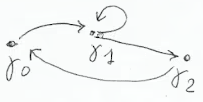
\includegraphics[width=10cm]{rappr_grafica_grafo.png}
    \end{center}
    Questa è una rappresentazione grafica di un grafo in cui i nodi sono gli stati e gli archi le transizioni
}

Se voglio definire la semantica (se voglio usare questo tipo di struttura) del linguaggio con la sintassi definita prima occorre definire uno stato di transazione specifico per \texttt{Exp}, per \texttt{Bexp} e per \texttt{Com}

Vi sono tuttavia \red{diversi problemucci}, del tipo:
\begin{enumerate}
    \item $\Gamma$ è di solito un insieme infinito contabile, allora vi è la \red{necessità di trovare una rappresentazione finita ed implicita attraverso grammatiche}. Questo vuol dire che $\Gamma$ coincide con uno dei linguaggi delle 3 categorie sintattiche (ovvero \texttt{Exp}, \texttt{Bexp}, \texttt{Com})
    \esempio{
        \[
            \Gamma_e = \{\langle e,\sigma \rangle | e \in Exp, \sigma \in Store\}
        \]
        Dove $\sigma$ è una funzione che associa ad ogni variabile un numero naturale, perché lo stato del mio sistema è una coppia in cui la prima parte indica l'espressione che devo valutare, la seconda componente è lo store che indica il valore dell'espressione   
    }
    \item $\rightarrow \subseteq \Gamma\times\Gamma$ è una relazione costituita da infinite coppie $\gamma \rightarrow \gamma'$, anche qui vi è la necessità di trovare una rappresentazione finita ed implicita come minima relazione che soddisfa \red{un certo insieme finito di assiomi e regole di inferenza}, quindi la semantica non è che un insieme di regole di inferenza che mi indicano in modo calcolare le transizioni che mi portano ad eseguire un certo comando
    \item per dare significato alle variabili (che posono solo assumere valore su $\mathbb{N}$) è necessario introdurre uno \textbf{store} $\sigma:Var\rightarrow \mathbb{N}$, come funzione che associa ad ogni variabile un valore
    \[
        \sigma = \{x_1/n_1, x_2/n_2, \dots, x_k/n_k\}    
    \]
    Se supponiamo che $var = \{x_1, x_2, \dots, x_k\}$
\end{enumerate}

\subsection{Semantica delle espressioni artimetiche}
Adesso introduciamo la \textbf{Semantica delle espressioni aritmetiche}, un tipo di semantica operazionale. Deve ovviamente avere un sistema di transizione $\langle \Gamma_e, T_e, \rightarrow_e \rangle$ dove:
\begin{itemize}
    \item $\Gamma_e = \{ \langle e, \sigma \rangle | e \in Exp, \sigma\in Store\}$
    \item $T_e = \{ \langle n, \sigma \rangle | n \in \mathbb{N}, \sigma\in Store\}$
    \item La relazione $\rightarrow_e$ è definita come la minima relazione che soddisfa gli assiomi e le regole di inferenza qui sotto:
    \begin{enumerate}
        \item \textbf{Variabile}:
        \[
        \frac{}{\langle v, \sigma \rangle \rightarrow_e \langle \sigma(v), \sigma \rangle}    
        \]
        Ovvero il tuo stato terminale sarà il numero della variabile $v$ indicato dallo Store (inoltre $\sigma$ rimane inalterato). Quindi valuto ciò che $v$ vale in $\sigma$
        \item \textbf{Somma 1}:
        \[
            \frac{\langle e_0, \sigma \rangle \rightarrow_e \langle e_0', \sigma' \rangle}{\langle e_0 + e_1, \sigma \rangle \rightarrow_e \langle e_0' + e_1, \sigma' \rangle}
        \]

        Nel momento in cui riesco a fare un passo di valutazione da $e_0$ a $e_0'$ alterando anche lo stato dello store da $\sigma$ a $\sigma'$ questa trasformazione si anche applicare durante una somma, in altre parole l’espressione si semplifica o riduce (ad esempio, una variabile viene sostituita con il suo valore), e nel contempo lo stato della memoria potrebbe essere aggiornato se l’espressione stessa comporta una modifica ai valori delle variabili

        \item \textbf{Somma 2}:
        \[
            \frac{\langle e_1, \sigma \rangle \rightarrow_e \langle e_1', \sigma' \rangle}{\langle m + e_1, \sigma \rangle \rightarrow_e \langle m + e_1', \sigma' \rangle}
        \]
        Stessa roba ma con un numero $m$
        \item \textbf{Somma 3}:
        \[
            \frac{}{\langle m+m', \sigma \rangle \rightarrow_e \langle P, \sigma \rangle}   \quad \text{ dove } P = m+m' 
        \]
        \item \textbf{Sottrazione 1}:
        \[
            \frac{\langle e_0, \sigma \rangle \rightarrow_e \langle e_0', \sigma' \rangle}{\langle e_0 - e_1, \sigma \rangle \rightarrow_e \langle e_0' - e_1, \sigma' \rangle}
        \]
        \item \textbf{Sottrazione 2}:
        \[
            \frac{\langle e_1, \sigma \rangle \rightarrow_e \langle e_1', \sigma' \rangle}{\langle m - e_1, \sigma \rangle \rightarrow_e \langle m - e_1', \sigma' \rangle}
        \]
        \item \textbf{Sottrazione 3}:
        \[
            \frac{}{\langle m - m', \sigma \rangle \rightarrow_e \langle p, \sigma \rangle}
        \]
        
   

    \end{enumerate}

    Si noti come la somma e la sottrazione prima valutano la sottoespressione di sinistra ($e_0$) con somma/sottrazione 1 poi, se questa s'è mutata in numero, valutano la sottoespressione di destra ($e_1$) con somma/sottrazione 2 ed infine, se questa s'è mutata in un numero, viene fatta la somma/sottrazione finale con somma/sottrazione 3

    \esempio{
        Esempietto per valutare $\langle (x+2)-y, \{x/5, y/3\} \rangle$:
        
        \begin{center}
            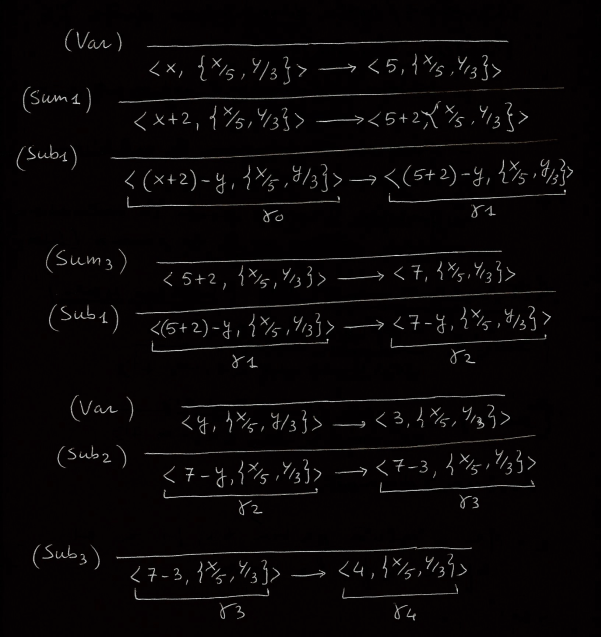
\includegraphics[width=10cm]{esempio_di_transizione.png}
        \end{center}

        Si ha, quindi, che $\gamma_0\rightarrow\gamma_1\rightarrow\gamma_2\rightarrow\gamma_3\rightarrow\gamma_4\in T_e$ cioè $\langle (x+2)-y, \{x/5, y/3\} \rangle \rightarrow^*\langle 4, \{x/5, y/3\} \rangle$
    }
\end{itemize}

\teorema{
    Vogliamo dimostrare che $\rightarrow_e$ è deterministico, ovvero:
    \[
        \gamma\rightarrow_e\gamma'\text{ e } \gamma\rightarrow_e\gamma''\text{, allora }\gamma'=\gamma''\quad \forall \gamma,\gamma',\gamma''  
    \]

    In altre parole significa che \red{da ogni transizione esce al più una transizione}, mai più di una
}
\pf{dimostrazione}{
    mi riduco a dimostrare che $(\inside{e,\sigma}\rightarrow_e \gamma' \land \inside{e,\sigma}\rightarrow_e\gamma'')\Rightarrow\gamma'=\gamma''$ 

    Procedo per induzione strutturale, con HP $(\inside{e,\sigma}\rightarrow_e \gamma' \land \inside{e,\sigma}\rightarrow_e\gamma'')\Rightarrow\gamma'=\gamma''$.
    \begin{enumerate}
        \item $e=m\in \mathbb{N}$: se $\inside{e,\sigma}\nrightarrow_e e$ allora la conclusione è vera perché la premessa è falsa
        \item $e=v\in Var$: Per la regola (Var), l'unica transizione derivabile per $\inside{v,\sigma}$ è $\inside{v,\sigma}\rightarrow_e \inside{\sigma(v), \sigma}$ poiché $\sigma$ è una funzione (cioè $\sigma(v)$ è univoco) e la sola regola (Var) è applicabile allora per forza $\inside{\sigma(v), \sigma} = \sigma'$ e $\inside{\sigma(v), \sigma}=\sigma''$ quindi $\gamma'=\gamma''$
        \item $e = e_0 + e_1$:
            Supponiamo che $\inside{e_0+e_1,\sigma}\rightarrow\gamma'$ e $\inside{e_0+e_1,\sigma}\rightarrow\gamma''$
            
            Ci sono 3 sottocasi da esaminare in accordo nel modo in cui derivo  $\inside{e_0+e_1,\sigma}\rightarrow\gamma'$:
            \begin{enumerate}
                \item  $\inside{e_0,\sigma}\rightarrow\inside{e_0',\sigma'}$ e $\gamma'=\inside{e_0' + e_1, \sigma'}$
                in questo caso ho che $e_0 \notin \mathbb{N}$ e la regola che ho applicato è \texttt{Somma 1}. 
                Allora se $\inside{e_0+e_1, \sigma}\rightarrow \gamma''$ è necessario che $\inside{e_0, \sigma}\rightarrow \inside{e_0'', \sigma''}$ e che $\gamma''=\inside{e_0''+e_1, \sigma''}$.

                Tuttavia per (HP) si ha che $\inside{e_0',\sigma'} = \inside{e_0'',\sigma''}$ pertanto deve essere che $e_0' = e_0''$ e $\sigma' = \sigma''$, da cui discende $\gamma' = \gamma''$
                \item $e_0 = m \in \mathbb{N}$ ed $\inside{e_1, \sigma}\rightarrow\inside{e_1', \sigma'}$ 
                Caso analogo al precedente, dato che ho che $e_1\notin\mathbb{N}$ e la regola che ho applicato è \texttt{Somma 2}. Allora se $\inside{e_0 + e_1, \sigma}\rightarrow \gamma''$, è necessario che $\inside{e_1, \sigma}\rightarrow \inside{e_1'',\sigma''}$ e $\gamma'' = \inside{e_0+e_1'',\sigma''}$. Tuttavia per (HP) si ha che $\inside{e_1',\sigma'} = \inside{e_1'',\sigma''}$ pertanto deve essere che $e_1' = e_1''$ e $\sigma' = \sigma''$, da cui discende $\gamma' = \gamma''$
                \item $e_0 \in \mathbb{N}$ ed $e_1\in \mathbb{N}$
                In questo caso, solo \texttt{Somma 3} è applicabile, ottenendo una sola passibile transizione:
                \[
                    \inside{e_0+e_1,\sigma} \to\inside{P, \sigma} \text{ dove } P = e_0+e_1
                \] 
                Quindi la tesi segue:
                \[
                    \inside{e_0+e_1,\sigma}\to\gamma'\land \inside{e_0+e_1,\sigma}\to\gamma''\implies\gamma'=\gamma''
                \]
            \end{enumerate}

            \item $e=e_1-e_2$: DEL TUTTO ANALOGO AL CASO PRECEDETE
            

            
        
    \end{enumerate}
    Q.e.d.
}

Questo teorema ci porta ad un dio boia di corollario:

\cor{}{
        poiché $\to_e$ è determinisca, a partire da $\inside{e,\sigma}$ arriveremo su una sola configurazione terminale $\inside{n,\sigma}$: "n è il valore di $e$ in $\sigma$"

        È possibile perciò definire una funzione 
        \[
            eval : Expr\times Store \dashrightarrow  \mathbb{N} 
        \]
        che da semantica alle espressione
        \[
            eval (e, \sigma) = \begin{cases}
                m & \text{ se }\inside{e,\sigma}\to^* \inside{m,\sigma}  \\
                \text{indefinita} & \text{altrimenti}
            \end{cases}   
        \]
}

Esempi:
\esempio{
    \begin{itemize}
        \item $eval((x+2)- y, \{x/5, y/3\}) = 4$ dato che
        \[
            \inside{(x+2)-y, \{x/5, y/3\}} \to^* \inside{4, \{x/5, y/3\}}    
        \]
        \item $eval((x+2)-y, \{x/2, y/7\})=indefinito$ dato che
        \[
            \inside{(x+2)-y, \{x/2, y/7\}} \to^* \inside{4-7, \{x/2, y/7\}} \nrightarrow     
        \]
    \end{itemize}
}

Inoltre sia introdotta la definizione di equivalenza:
\dfn{Equivalenza tra espressioni}{
    Siano $e$ ed $e'$ due espressioni, allora si dicono \textbf{equivalenti} sse $\forall\sigma\in Store \quad eval(e,\sigma)=eval(e',\sigma)$

    E si denota con $e \equiv e'$
}
Esempietto:
\esempio{
    $v_1+(v_2+v_3)\equiv(v_1 + v_2) + v_3$
}

Si osservi come \texttt{Eval} è definita rispetto alla disciplina di valutazione \texttt{IS} (interno destro), pertanto, rigorosamente, \texttt{Eval} è denotato come $Eval_{is}$. Si può, inoltre, dimostrare che anche per \texttt{ID} (interno destro), il risultato della valutazione è lo stesso:
\[
    Eval_{is} = Eval_{id}    
\]

Dove $Eval_{id}(e,\sigma) = \begin{cases} m & \text{ se }\inside{e,\sigma}\to^*_{id} \inside{m,\sigma}  \\ \text{indefinita} & \text{altrimenti}\end{cases}$

Come vedremo, è possibile definire anche altre siscipline di valutazione come Esterna Sinistra, Esterne Destra, Esterna parallela.
\subsection{Semantica delle espressioni booleane}
Arriviamo alle espressioni booleane con la seguente grammatica:
\[
    b ::= t|e=e|b\text{ or }b| \lnot b    
\]
(ricordo che $t$ è una metavariabile con un valore di verità true o false)
E il seguente sistema di transazione:
\[
    \inside{\Gamma_b, T_b, \to_b} \text{ dove } \Gamma_b = \{\inside{b,\sigma}|b\in Bexp, \sigma\in Store\} \text{ e } T_b=\{\inside{tt,\sigma}, \inside{ff,\sigma}| \sigma\in Store\}    
\]

e $\to_b$ è la minima relazione generata dai seguenti assiomi e regole di inferenza:
\begin{itemize}
    \item \textbf{Eq1} 

    \[
        \frac{\langle e_0 = e_1, \sigma \rangle \to_b \langle e_1', \sigma' \rangle}{\langle m = e_1, \sigma \rangle \to_b \langle m = e_1', \sigma' \rangle}
    \]
    \item \textbf{Eq2}
    \[
        \frac{\inside{e_1, \sigma}\to_e\inside{e_1',\sigma'}}{\langle m = e_1, \sigma \rangle \to_b \langle m = e_1', \sigma' \rangle}
    \]
    \item \textbf{Eq3}
    \[  
        \frac{}
        {\langle m = m, \sigma \rangle \to_b \langle t, \sigma \rangle} \text{ dove } t = \begin{cases} 
            \text{tt} & \text{se } m = n \\
            \text{ff} & \text{se } m \neq n 
        \end{cases}  
    \]
    \item \textbf{Or1}
    \[
        \frac{\inside{b_0,\sigma}\to_b\inside{b_0',\sigma'}}{\inside{b_0 \text{ or }b_1,\sigma} \to_b \inside{b_0' \text{ or }b_1, \sigma'}}  
    \]
    \item \textbf{Or2}
    \[
        \frac{}{\inside{tt \text{ or }b_1, \sigma}\to_b\inside{tt, \sigma}}    
    \]
    \item \textbf{Or3}
    \[
        \frac{}{\inside{ff \text{ or } b_1, \sigma}\to_b \inside{b_1,\sigma}}    
    \]
    \item \textbf{Neg1}
    \[
        \frac{\inside{b,\sigma}\to_b\inside{b', \sigma'}}{\inside{\lnot b, \sigma}\to_b\inside{\lnot b', \sigma'}}    
    \]
    \item \textbf{Neg2}
    \[
        \frac{}{\inside{\lnot b, \sigma}\to_b\inside{t', \sigma}}\text{ dove }t' = \begin{cases}
            tt \text{ se }t=ff
            ff \text{ se }t=tt
        \end{cases}  
    \]
\end{itemize}

Si tenga presente che \texttt{Eq1}, \texttt{Eq2} e \texttt{Eq3} sono cosiddette \textbf{interne sinistre} perché inizio a valutare la sottoespressione di sinistra per poi restituire un valore di verità $t$ sse ho ottenuto numeri in tutte e due le sottoespressioni mentre  \texttt{Or1}, \texttt{Or2} e \texttt{Or3} sono \textbf{esterne sinistre} perché inizio a valutare la sottoespressione di sinistra per poi restituire un valore di verità $t$ sse ho ottenuto numeri almeno in una sottoespressione. Quindi se nelle interne dovevo avere dei numeri in tutte le sottoespressioni per poi eseguire la valutazione finale nelle esterne per eseguire la valutazione finale mi basta avere una quantità sufficiente

Anche per i booleani si ha questo teorema:
\teorema{
    $\to_b$ è deterministica, ovvero 
    \[
        (\gamma \to_b \gamma' \land \gamma\to_b\gamma'')\implies \gamma' = \gamma''    
    \]
}
Che porta al seguente corollario:
\cor{}{
    si può, quindi, definire:
    \[
        eval_b(b,\sigma) = \begin{cases}
            t & \text{se }\inside{b,\sigma}\to^*\inside{t,\sigma}\\
            \text{indefinita} & \text{altrimenti}
        \end{cases}       
    \]
}

E si ha anche la seguente definizione:
\dfn{Equivalenza booleani}{
    Siano $b$ ed $b'$ due booleani, allora si dicono \textbf{equivalenti} sse $\forall\sigma\in Store \quad eval_b(b,\sigma)=eval_b(b',\sigma)$

    E si denota con $b \equiv b'$
}
\esempio{
    \[
        \lnot((3=v)\lor (3=4)) = \lnot(v=3)       
    \]
}

Si possono definire per $b_0$ or $b_1$ regole di valutazioni diverse da \texttt{ES}. Ad esempio \texttt{ED} o \texttt{IS}, ma non sono tutte equivalenti, si provi, ad esempio, con \texttt{ED}:

\begin{itemize}
    \item \textbf{Or1'}:
    \[\frac{\inside{b_1, \sigma}\to_b\inside{b_1',\sigma'}}{\inside{b_0 \text{ or }b_1, \sigma}\to_b\inside{b_0 \text{ or } b_1', \sigma'}}\]
    \item \textbf{Or2'}:
    \[
        \frac{}{\inside{b_0 \text{ or }tt, \sigma}\to_b \inside{tt, \sigma}}    
    \]
    \item \textbf{Or3'}:
    \[
        \frac{}{\inside{b_0 \text{ or }ff, \sigma}\to_b \inside{b_0, \sigma}}    
    \]
\end{itemize}
\esempio{
    $\gamma=\inside{}$
}
  
